\documentclass[UTF8,aspectratio=1610,10pt]{ctexbeamer}
\usepackage{latexsym}
\usepackage{amsmath,amssymb}
\usepackage{color,xcolor}
\usepackage{graphicx}
\usepackage{algorithm}
\usepackage{amsthm}
% enable full XeLaTeX power
\usepackage{xltxtra}
\usepackage{multirow}
\usepackage{tabularx}
\usepackage{booktabs}
\usepackage{fontawesome}
\usetheme{Berlin}
%\usetheme{CambridgeUS}
\usefonttheme[onlymath]{serif}
\usecolortheme{beaver}

\newtheorem{proposition}[theorem]{命题}
\setbeamertemplate{theorems}[numbered]
\begin{document}

\title[Blood Diseases Diagnosis]{血液疾病辅助诊断方法研究}
\author[ ]{ }
\institute[math]{}
\date[ ]{\today}
\frame{\titlepage}

\begin{frame}
\frametitle{血液样本数据指标项}

\section{背景}

\begin{table}
\centering
\caption{血常规指标项(正负样本字段)}
\begin{tabular}{|l|l||l|l|}
\toprule
指标项	&	统一字段名 & 指标项	&	统一字段名 \\
\midrule
平均血红蛋白含量	&	MCH	&	中性粒细胞比率	&	NEUT\_P	\\
平均血红蛋白浓度	&	MCHC	&	中性粒细胞计数	&	NEUT	\\
红细胞平均体积	&	MCV	&	血小板压积	&	PCT	\\
平均血小板体积	&	MPV	&	\underline{红细胞分布宽度}	&	\underline{RDW}	\\
嗜碱性粒细胞计数	&	BAS	&	淋巴细胞计数	&	LY	\\
嗜碱性粒细胞比率	&	BAS\_P	&	淋巴细胞比率	&	LY\_P	\\
嗜酸性粒细胞计数	&	EOS	&	单核细胞计数	&	MONO	\\
嗜酸性粒细胞比率	&	EOS\_P	&	单核细胞比率	&	MONO\_P	\\
血红蛋白	&	HB	&	红细胞计数	&	RBC	\\
血小板分布宽度	&	PDW	&	红细胞压积	&	HCT	\\
血小板计数	&	PLT	&	性别	&	Sex	\\
白细胞计数	&	WBC	&	年龄	&	Age	\\
诊断结果	&	Result	&		&	\\
\bottomrule
\end{tabular}
\end{table}

\end{frame}

\begin{frame}
\frametitle{正样本数据}
\begin{table}
\caption{疾病分类汇总数据}
\centering
\begin{tabular}{|l|l|r|}
\toprule
疾病分类	& 英文对照	&总数	\\
\midrule
淋巴瘤	& Lymphoma &	5202	\\
多发性骨髓瘤[卡勒病] (M97320/3)	&	&2183	\\
急性髓样白血病	&	&2051	\\
血小板减少性紫癜	&	&1155	\\
急性淋巴细胞白血病	&	&1154	\\
过敏性紫癜[亨诺克(-舍恩莱因)紫癜]	&	&1105	\\
再生障碍性贫血 NOS	&	&458	\\
噬血细胞综合症	&	&374	\\
骨髓增生异常综合征	&	&229	\\
\bottomrule
合计	&	&13911	\\
\bottomrule
\end{tabular}
\end{table}
\end{frame}

\begin{frame}
\frametitle{负样本数据}
合计:728,599
\end{frame}

\begin{frame}
\frametitle{实验流程}
\begin{enumerate}
  \item 样本比例
	\begin{itemize}
	  \item 1 : 1
	  \item 1 : 2
	  \item 1 : 5
	  \item 1 : 10
	\end{itemize}
  \item 训练模型
	  \begin{itemize}
		  \item 逻辑回归
		  \item 随机森林
		  \item Light GBM
		  \item XGBoost
		  \item 神经网络
		\end{itemize}
  \item 记录结果参数与过程
\end{enumerate}

\end{frame}

\section{Problems}
\subsection{Samples}

\begin{frame}
\frametitle{Imbalanced Class Distribution(aka. Skewed Class)}
\begin{itemize}
  \item Challenges with Standard Machine Learning Techniques
  

  \item Resampling Techniques
  \item Algorithmic Ensemble Techniques
  
\end{itemize}
\end{frame}

\subsection{Imbalanced Data}

\begin{frame}
\frametitle{Resampling Techniques}
\begin{itemize}
\item Random Under-Sampling: randomly \textbf{eliminate} \textbf{majority} class examples
\begin{itemize}
  \item[\faThumbsOUp] improve run time and storage problems
  \item[\faThumbsODown] information loss \& biased sample
\end{itemize}

\item Random Over-Sampling: randomly \textbf{replicate} instances in the \textbf{minority} class 
  	\begin{itemize}
  	\item[\faThumbsOUp] no information loss \& Outperforms under sampling
  	\item[\faThumbsODown] overfitting
	\end{itemize}
	
\item Cluster-Based Over Sampling: K-means clustering
\item Informed Over Sampling: Synthetic Minority Over-sampling Technique
\begin{itemize}
  \item[\faThumbsOUp] Mitigates overfitting \& No loss of useful information
  \item[\faThumbsODown] SMOTE can introduce additional noise \& is not very effective for high dimensional data
\end{itemize}

\item Modified synthetic minority oversampling technique (MSMOTE)
\begin{itemize}
  \item Security/Safe samples: k nearest neighbors
  \item Border samples: nearest neighbor
  \item Latent nose samples: nothing
\end{itemize}
\end{itemize}
\end{frame}

\section{Machine Learning Model}
\begin{frame}
\frametitle{P vs NP,二分类,Train 1:1 , Test 1:1000, Random Forest}
\begin{figure}
\centering
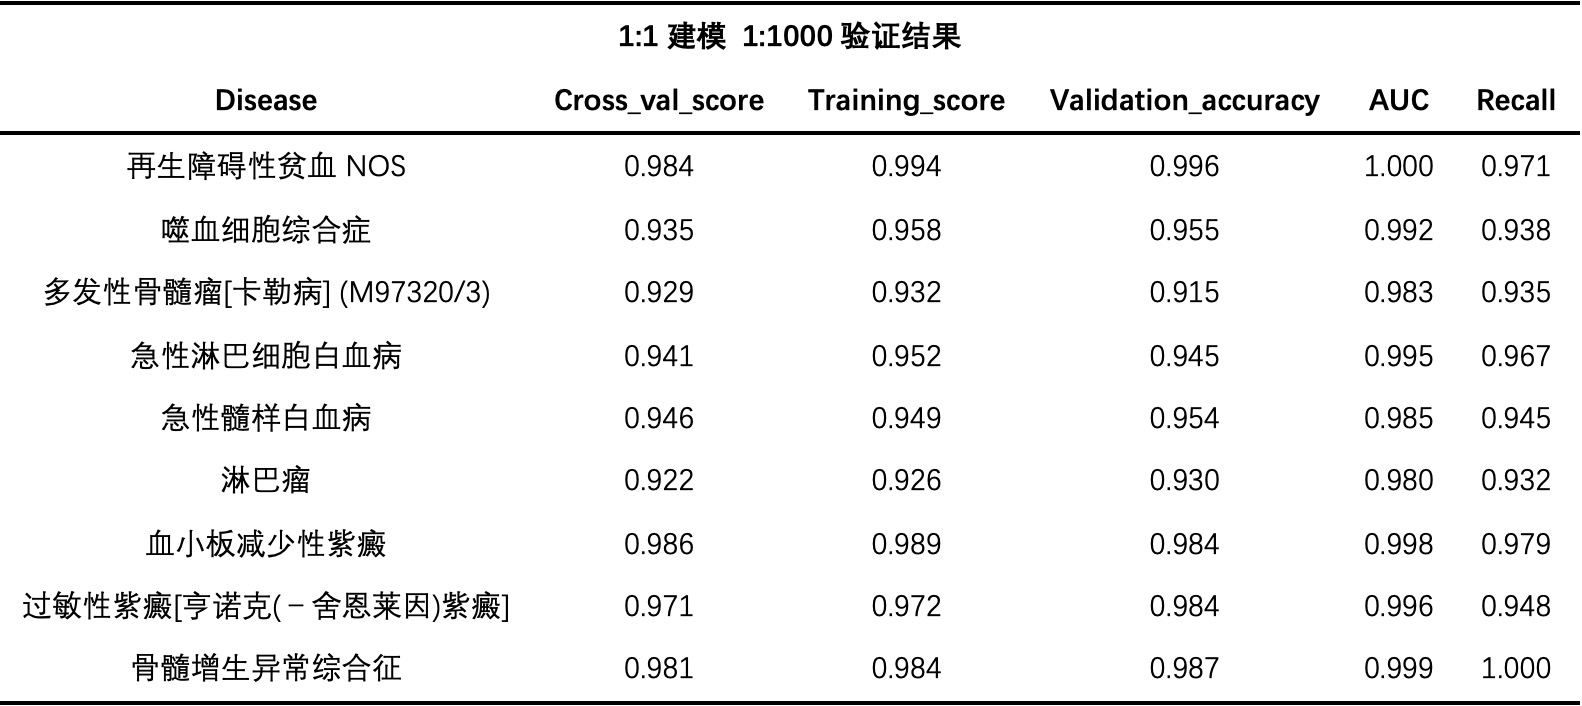
\includegraphics[width=\textwidth]{images/1to1-1t1000.jpg}	
\end{figure}
\end{frame}

\begin{frame}
\frametitle{P vs NP,二分类,Train 1:1 , Test 1:1000, XGBoost}
\begin{figure}
\centering
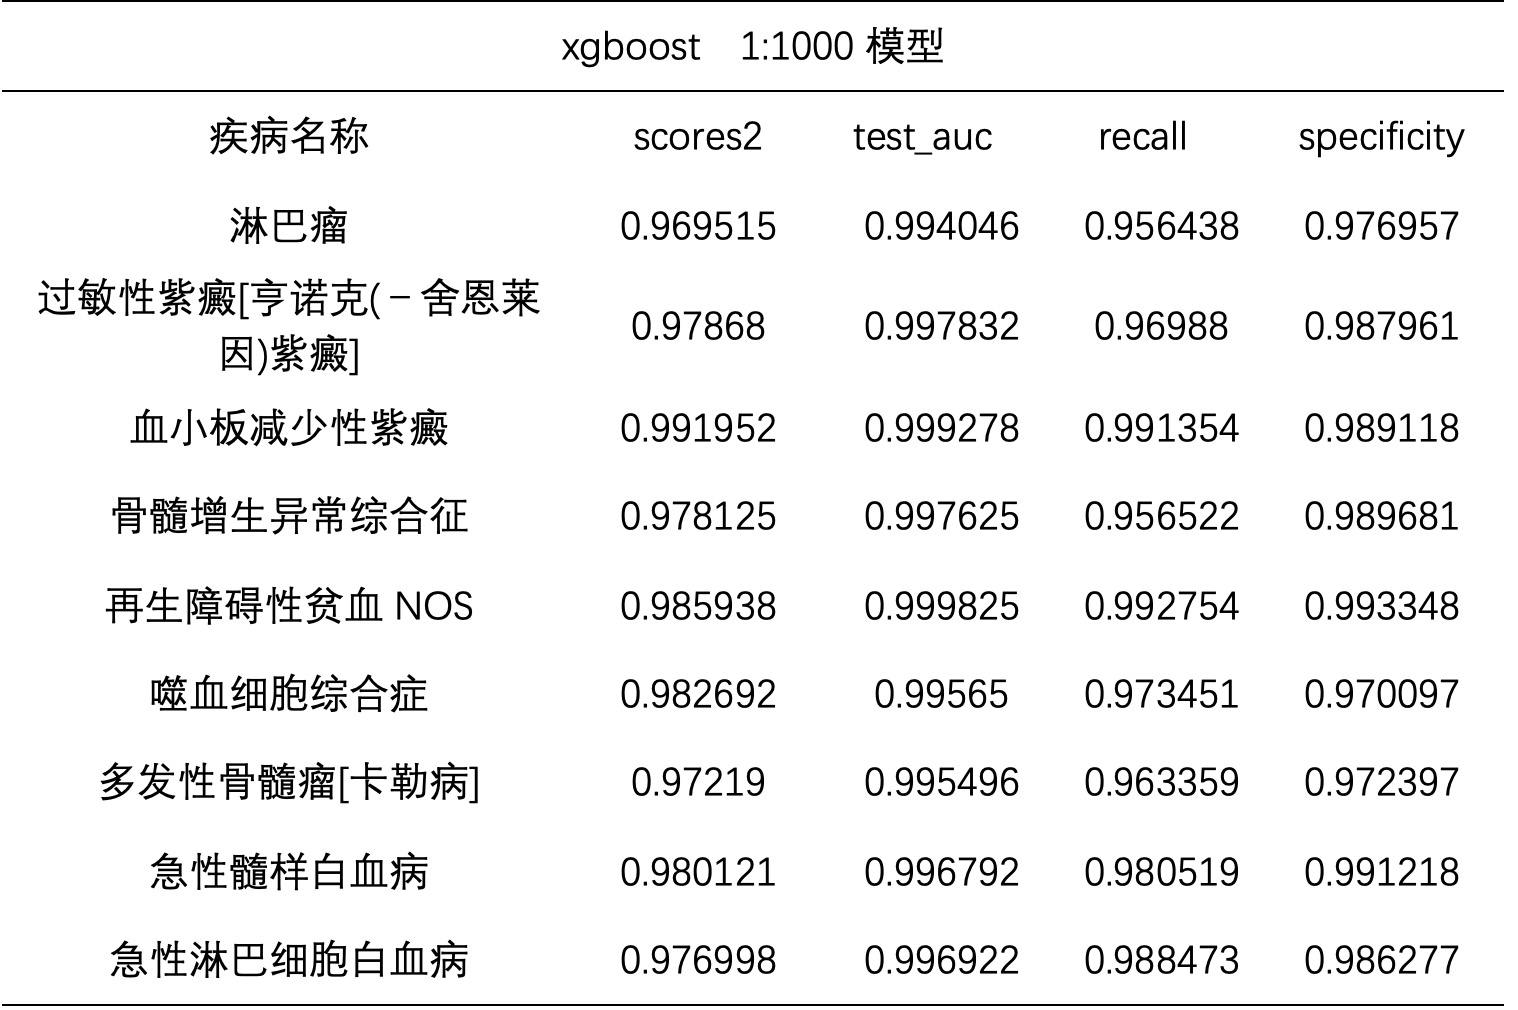
\includegraphics[width=.75\textwidth]{images/xgboost-1t1000.jpg}	
\end{figure}
\end{frame}


\section{Prevalence of Blood Disorders}

\begin{frame}
\frametitle{患病率}
\begin{table}
	\centering

\begin{tabular}{l|rr|r}

疾病	& 患病数	& 统计人群数	& 患病率(10万)\\

\hline
噬血细胞综合症	& 77	& 5156988	& 1.493119627\\

再生障碍性贫血	& 3316	& 5156982	& 64.3011746\\

血小板减少性紫癜	& 256	& 5156990	& 4.964136056\\

过敏性紫癜	& 1075	& 5156988	& 20.84550129\\

骨髓增生异常综合症	& 315	& 5156988	& 6.108216657\\

急性淋巴细胞白血病	& 134	& 5156988	& 2.598415975\\

急性髓样白血病	& 29	& 5156988	& 0.562343756\\

多发性骨髓瘤	& 727	& 5156988	& 14.09737622\\

淋巴瘤	& 89	& 5156988	& 1.725813595\\
\hline
合计	& 6018	&	& 116.6960978\\

\end{tabular}
\end{table}
\end{frame}

\section{血液病诊断云平台}

\begin{frame}
\begin{figure}
	\centering
	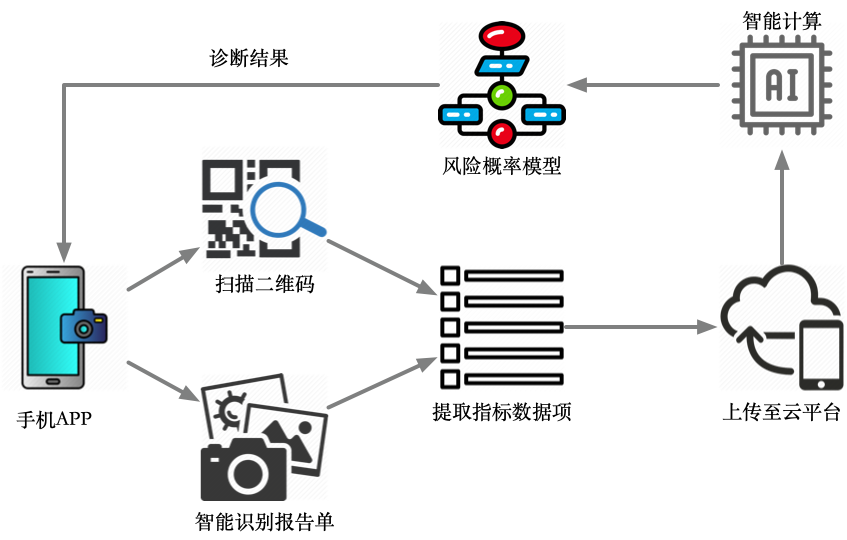
\includegraphics[width=.9\textwidth]{images/prototype.png}
\end{figure}
\end{frame}


\end{document}